%And then the actual code for creating the figure:
\documentclass{standalone}
\usepackage{tikz}
\usetikzlibrary{arrows}
\begin{document}

% First, set the overall layout of the tree
% You might need to play with these sizes to ensure nothing overlaps.
\tikzstyle{level 1}=[level distance=1.1cm, sibling distance=2.8cm]
\tikzstyle{level 2}=[level distance=1.1cm, sibling distance=1.5cm]
\tikzstyle{level 3}=[level distance=1.1cm, sibling distance=1.4cm]
\tikzstyle{level 4}=[level distance=1.1cm, sibling distance=2cm]
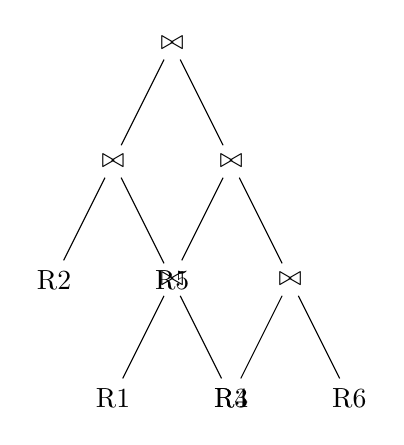
\begin{tikzpicture}
% Start with the parent node, 
% and slowly build out the tree
% with each "child" representing 
% a new level of the diagram
% each "node" represents a labelled 
% (or unlabeled if you 
% want) node in the diagram.
\node {$\bowtie$}
    child{
        node{$\bowtie$}
        child{
          % Put the name of the node in parenthesis
       	  % for reference later. 
       	  % The label shown in the diagram
          % goes in the brackets. 
          % This label can use math mode.
            node{R2}
            edge from parent
            node[left]{}
        }
        child {
            node(a){$\bowtie$}
            child{
                node{R1}
                edge from parent
                node[left]{}
            }
            child{
                node{R3}
                edge from parent
                node[right]{}
            }
            edge from parent
            node[right]{}
        }
        edge from parent
        node[left]{}
    }
    child{
        node{$\bowtie$}
        child{
          % Put the name of the node in parenthesis
       	  % for reference later. 
       	  % The label shown in the diagram
          % goes in the brackets. 
          % This label can use math mode.
            node{R5}
            edge from parent
            node[left]{}
        }
        child {
            node{$\bowtie$}
			child{
                node{R4}
                edge from parent
                node[left]{}
            }
            child{
                node{R6}
                edge from parent
                node[right]{}
            }            
            edge from parent
            node[right]{}
        }
        edge from parent
        node[right]{}
    };
%Now I create the information set. Note that I utilize the names
%that I had previously assigned to nodes in my graph
%\draw [dashed](a)--(b);
%\draw [dashed](b)--(c);
\end{tikzpicture}
\end{document}